\section{Methodology}
We use different feature sets and machine learning classifiers to determine the
best combination for sentiment analysis of twitter. We also experiment with
various pre-processing steps like -- punctuations, emoticons, twitter specific
terms and stemming.  We investigated the following features -- unigrams,
bigrams, trigrams and negation detection. We finally train our classifier using
various machine-learning algorithms -- Naive Bayes, Decision Trees and Maximum
Entropy.

\begin{figure}[h!]
\centering
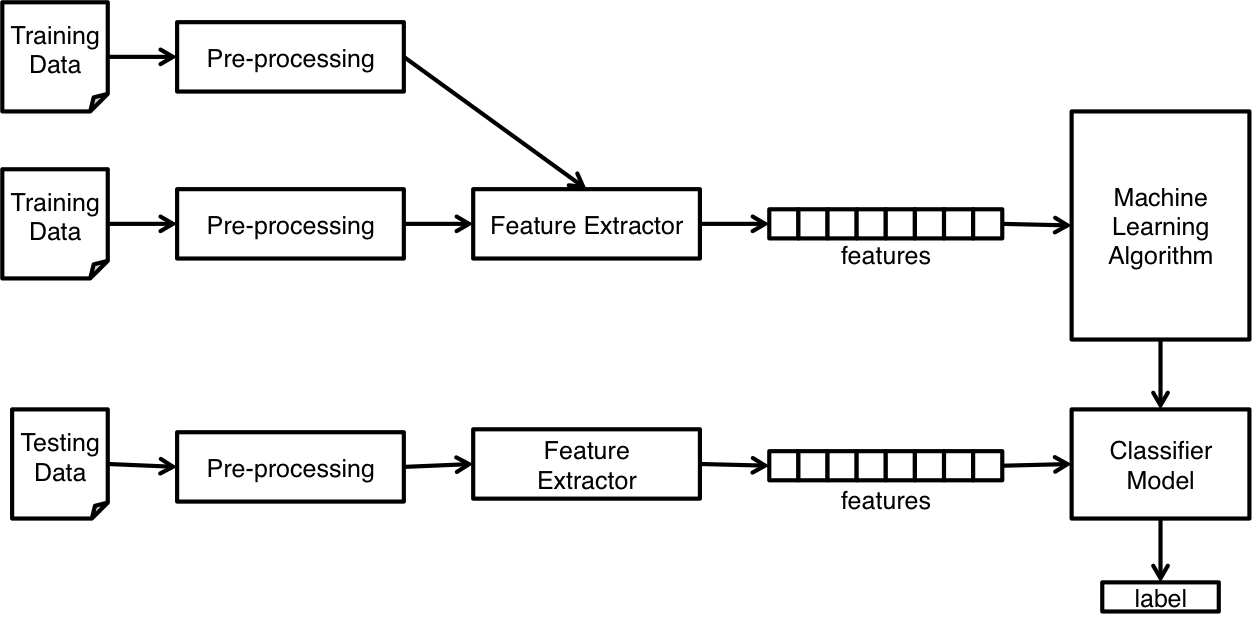
\includegraphics[width=0.75\textwidth]{img/schematic.png}
\caption{Schematic Diagram of Methodology}
%TODO Lame caption?
\label{fig:schematic}
\end{figure}

We use a modularized approach with feature extractor and classification
algorithm as two independent components. This enables us to experiment with
different options for each component. \figref{fig:schematic} illustrates
different steps taken in the entire process.

\subsection{Datasets}
One of the major challenges in Sentiment Analysis of Twitter is to collect a
labelled dataset. Researchers have made public the following datasets for
training and testing classifiers.

\subsubsection{Twitter Sentiment Corpus} This is a collection of 5513 tweets
collected for four different topics, namely, Apple, Google, Microsoft, Twitter
It is collected and hand-classified by Sanders Analytics LLC \cite{San}. Each
entry in the corpus contains, Tweet id, Topic and a Sentiment label. We use
Twitter-Python library to enrich this data by downloading data like Tweet text,
Creation Date, Creator etc. for every Tweet id. Each Tweet is
hand classified by an American male into the following four categories. For the
purpose of our experiments, we consider Irrelevant and Neutral to be the same
class. Illustration of Tweets in this corpus is show in \tabref{tab:TSC}.
%TODO \cite{TwPyLib}

\begin{description}
	\item[Positive] {For showing positive sentiment towards the topic}
	\item[Positive] {For showing no or mixed or weak sentiments towards the topic}
	\item[Negative] {For showing negative sentiment towards the topic}	
	\item[Irrelevant] {For non English text or off-topic comments}
\end{description}

\begin{table}[h!]
\centering

\begin{tabular}{|l|r|p{0.75\textwidth}|}
\hline
Class & Count & Example \\\hline
neg & 529 & {{\#}Skype often crashing: {\#}microsoft, what are you doing?} \\\hline
neu & 3770 & {How {\#}Google Ventures Chooses Which Startups Get Its \$200
				Million http://t.co/FCWXoUd8 via @mashbusiness @mashable} \\\hline
pos & 483 & {Now all @Apple has to do is get swype on the iphone and
				it will be crack. Iphone that is} \\\hline

\end{tabular}

\caption{Twitter Sentiment Corpus}
\label{tab:TSC}
\end{table}

\subsubsection{Stanford Twitter} This corpus of tweets, developed by Sanford’s
Natural Language processing research group, is publically available \cite{GBH}.
The training set is collected by querying Twitter API for happy emoticons like
``\texttt{:)}'' and sad emoticons like ``\texttt{:(}'' and labelling them
positive or negative. The emoticons were then stripped and Re-Tweets and
duplicates removed. It also contains around 500 tweets manually collected and
labelled for testing purposes. We randomly sample and use 5000 tweets from this
dataset. An example of Tweets in this corpus are shown in \tabref{tab:STAN}.

\begin{table}[h!]
\centering

\begin{tabular}{|l|r|p{0.75\textwidth}|}
\hline
Class & Count & Example \\\hline
neg & 2501 & Playing after the others thanks to TV scheduling may well allow us to know what's go on, but it makes things look bad on Saturday nights  \\\hline
pos & 2499 & @francescazurlo HAHA!!! how long have you been singing that song now? It has to be at least a day. i think you're wildly entertaining!  \\\hline

\end{tabular}

\caption{Stanford Corpus}
\label{tab:STAN}
\end{table}


\subsection{Pre Processing} User-generated content on the web is seldom present
in a form usable for learning. It becomes important to normalize the text by
applying a series of pre-processing steps. We have applied an extensive set of
pre-processing steps to decrease the size of the feature set to make it suitable
for learning algorithms. \figref{fig:tweet} illustrates various
features seen in micro-blogging. \tabref{tab:feat_freq} illustrates the frequency of these
features per tweet, cut by datasets. We also give a brief description of pre-processing steps taken.

\begin{figure}[h!]
\centering
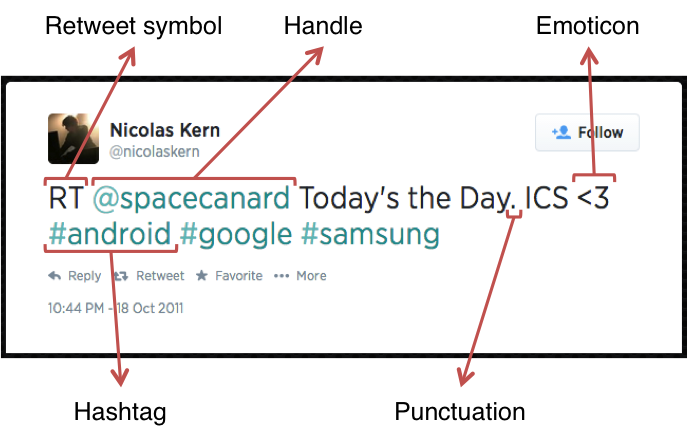
\includegraphics[width=0.75\textwidth]{img/tweet.png}
\caption{Illustration of a Tweet with various features}
\label{fig:tweet}
\end{figure}

\begin{table}[h!]
\centering

\begin{tabular}{|l|rr|rr|rr|}
\hline
 & \multicolumn{2}{c|}{Twitter Sentiment}
 & \multicolumn{2}{c|}{Stanford Corpus}
 & \multicolumn{2}{c|}{Both} \\\hline
Features	& \multicolumn{1}{c}{Avg.} & \multicolumn{1}{c|}{Max.}
			& \multicolumn{1}{c}{Avg.} & \multicolumn{1}{c|}{Max.}
			& \multicolumn{1}{c}{Avg.} & \multicolumn{1}{c|}{Max.} \\\hline
Handles		&  0.6761 &  8 &  0.4888 & 10 &  0.5804 & 10 \\
Hashtags	&  2.0276 & 13 &  0.0282 & 11 &  1.0056 & 13 \\
Urls		&  0.4431 &  4 &  0.0452 &  2 &  0.2397 &  4 \\
Emoticons	&  0.0550 &  3 &  0.0154 &  4 &  0.0348 &  4 \\
Words		& 14.4084 & 31 & 13.2056 & 33 & 13.7936 & 33 \\\hline

\end{tabular}

\caption{Frequency of Features per Tweet}
\label{tab:feat_freq}
\end{table}

\subsubsection{Hashtags} A hashtag is a word or an un-spaced phrase prefixed
with the hash symbol (\#). These are used to both naming subjects and phrases
that are currently in trending topics. For example, {\#}iPad, {\#}news

Regular Expression: \verb'#(\w+)'

Replace Expression: \verb'HASH_\1'

\subsubsection{Handles} Every Twitter user has a unique username. Any thing
directed towards that user can be indicated be writing their username preceded
by ‘@’. Thus, these are like proper nouns. For example, @Apple

Regular Expression: \verb'@(\w+)'

Replace Expression: \verb'HNDL_\1'

\subsubsection{URLs} Users often share hyperlinks in their tweets. Twitter
shortens them using its in-house URL shortening service, like
http://t.co/FCWXoUd8 -- such links also enables Twitter to alert users if the
link leads out of its domain. From the point of view of text classification, a
particular URL is not important. However, presence of a URL can be an important
feature. Regular expression for detecting a URL is fairly complex because of
different types of URLs that can be there, but because of Twitter’s shortening
service, we can use a relatively simple regular expression.

Regular Expression: \verb'(http|https|ftp)://[a-zA-Z0-9\./]+'

Replace Expression: \verb'URL'

\subsubsection{Emoticons} Use of emoticons is very prevalent throughout the web,
more so on micro-blogging sites. We identify the following emoticons and replace
them with a single word. \tabref{tab:emot} lists the emoticons we are currently
detecting. All other emoticons would be ignored.

\begin{table}[h!]
\centering
	\begin{tabular}{|l|llllll|}
	
	\hline
		\multicolumn{1}{|c|}{Emoticons} &
		\multicolumn{6}{c|}{Examples} \\
	\hline
	\verb+EMOT_SMILEY+ 	& \verb+:-)+ 	& \verb+:)+ 	& \verb+(:+ 	& \verb+(-:+ 	& \verb++ 	& \verb++ \\
	\verb+EMOT_LAUGH+ 	& \verb+:-D+ 	& \verb+:D+ 	& \verb+X-D+ 	& \verb+XD+ 	& \verb+xD+ 	& \verb++ \\
	\verb+EMOT_LOVE+ 	& \verb+<3+ 	& \verb+:*+ 	& \verb++ 	& \verb++ 	& \verb++ 	& \verb++ \\
	\verb+EMOT_WINK+ 	& \verb+;-)+ 	& \verb+;)+ 	& \verb+;-D+ 	& \verb+;D+ 	& \verb+(;+ 	& \verb+(-;+ \\
	\verb+EMOT_FROWN+ 	& \verb+:-(+ 	& \verb+:(+ 	& \verb+(:+ 	& \verb+(-:+ 	& \verb++ 	& \verb++ \\
	\verb+EMOT_CRY+ 	& \verb+:,(+ 	& \verb+:'(+ 	& \verb+:"(+ 	& \verb+:((+ 	& \verb++ 	& \verb++ \\
	\hline
	
	\end{tabular}
\caption{List of Emoticons}
\label{tab:emot}
\end{table}

\subsubsection{Punctuations} Although not all Punctuations are important from
the point of view of classification but some of these, like question mark,
exclamation mark can also provide information about the sentiments of the text.
We replace every word boundary by a list of relevant punctuations present at
that point. \tabref{tab:punc} lists the punctuations currently identified. We also
remove any single quotes that might exist in the text.

\begin{table}[h!]
\centering
	\begin{tabular}{|l|ll|}
	
	\hline
		\multicolumn{1}{|c|}{Punctuations} &
		\multicolumn{2}{c|}{Examples} \\
	\hline
	\verb+PUNC_DOT+ & \verb+.+ & \verb++ \\
	\verb+PUNC_EXCL+ & \verb+!+ & \verb+¡+ \\
	\verb+PUNC_QUES+ & \verb+?+ & \verb+¿+ \\
	\verb+PUNC_ELLP+ & \verb+...+ & \verb+…+ \\
	\hline

	\end{tabular}
\caption{List of Punctuations}
\label{tab:punc}
\end{table}

\subsubsection{Repeating Characters} People often use repeating characters while
using colloquial language, like ``I’m in a hurrryyyyy'', ``We won, yaaayyyyy!''
As our final pre-processing step, we replace characters repeating more than twice
as two characters.

Regular Expression: \verb'(.)\1{1,}'

Replace Expression: \verb'\1\1'

\subsubsection*{Reduction in feature space} It’s important to note that by
applying these pre-processing steps, we are reducing our feature set otherwise
it can be too sparse. \tabref{tab:reduction} lists the decrease in feature set
due to processing each of these features.

\begin{table}[h!]
\centering

\begin{tabular}{|l|rr|rr|rr|}
\hline
 & \multicolumn{2}{c|}{Twitter Sentiment}
 & \multicolumn{2}{c|}{Stanford Corpus}
 & \multicolumn{2}{c|}{Both} \\\hline
Preprocessing
			& \multicolumn{1}{c}{Words} & \multicolumn{1}{c|}{Percentage}
			& \multicolumn{1}{c}{Words} & \multicolumn{1}{c|}{Percentage}
			& \multicolumn{1}{c}{Words} & \multicolumn{1}{c|}{Percentage} \\\hline
None			& 19128 &         & 15910 &         & 31832 &         \\
Hashtags		& 18649 & 97.50\% & 15550 & 97.74\% & 31223 & 98.09\% \\
Handles			& 17118 & 89.49\% & 13245 & 83.25\% & 27383 & 86.02\% \\
Urls			& 16723 & 87.43\% & 15335 & 96.39\% & 29083 & 91.36\% \\
Emoticons		& 18631 & 97.40\% & 15541 & 97.68\% & 31197 & 98.01\% \\
Punctuations	& 13724 & 71.75\% & 11225 & 70.55\% & 22095 & 69.41\% \\
Repeatings		& 18540 & 96.93\% & 15276 & 96.02\% & 30818 & 96.81\% \\\hline
All				& 11108 & 58.07\% &  8646 & 54.34\% & 16981 & 53.35\% \\
\hline
\end{tabular}

\caption{Number of words before and after pre-processing}
\label{tab:reduction}
\end{table}


\subsection{Stemming Algorithms} All stemming algorithms are of the following
major types – affix removing, statistical and mixed. The first kind, Affix
removal stemmer, is the most basic one. These apply a set of transformation
rules to each word in an attempt to cut off commonly known prefixes and / or
suffixes \cite{Ilia}. A trivial stemming algorithm would be to truncate words at N-th
symbol. But this obviously is not well suited for practical purposes.

J.B. Lovins described first stemming algorithm in 1968. It defines 294 endings,
each linked to one of 29 conditions, plus 35 transformation rules\ignore{need to write
more, conditions, transformations?}. For a word being stemmed, an ending with a
satisfying condition is found and removed. Another famous stemmer used
extensively is described in the next section.

\subsubsection{Porter Stemmer}

Martin Porter wrote a stemmer that was published in July 1980. This stemmer was
very widely used and became and remains the de facto standard algorithm used for
English stemming. It offers excellent trade-off between speed, readability, and
accuracy. It uses a set of around 60 rules applied in 6 successive steps \cite{Porter}. An
important feature to note is that it doesn’t involve recursion. The steps in the
algorithm are described in \tabref{tab:porter}.

\begin{table}[h!]
\centering
\begin{tabular}{|r|l|} \hline
1.	&	Gets rid of plurals and -ed or -ing suffixes \\ \hline
2.	&	Turns terminal y to i when there is another vowel in the stem \\ \hline
3.	&	Maps double suffixes to single ones: -ization, -ational, etc. \\ \hline
4.	&	Deals with suffixes, -full, -ness etc. \\ \hline
5.	&	Takes off -ant, -ence, etc. \\ \hline
6.	&	Removes a final –e \\ \hline
\end{tabular}
\caption{Porter Stemmer Steps}
\label{tab:porter}
\end{table}

\ignore{Another commonly used algorithm is [blah]. Which does [blah].}

\subsubsection{Lemmatization}

Lemmatization is the process of normalizing a word rather than just finding its
stem. In the process, a suffix may not only be removed, but may also be
substituted with a different one. It may also involve first determining the
part-of-speech for a word and then applying normalization rules. It might also
involve dictionary look-up. For example, verb ‘saw’ would be lemmatized to ‘see’
and the noun ‘saw’ will remain ‘saw’. For our purpose of classifying text,
stemming should suffice.


\subsection{Features}
A wide variety of features can be used to build a classifier for tweets. The most widely used and basic feature set is word n-grams. However, there's a lot of domain specific information present in tweets that can also be used for classifying them. We have experimented with two sets of features:

\subsubsection{Unigrams}
Unigrams are the simplest features that can be used for text classification. A Tweet can be represented by a multiset of words present in it. We, however, have used the presence of unigrams in a tweet as a feature set. Presence of a word is more important than how many times it is repeated. Pang et al. found that presence of unigrams yields better results than repetition \cite{survey}. This also helps us to avoid having to scale the data, which can considerably decrease training time \cite{GBH}. \figref{fig:1grams} illustrated the cumulative distribution of words in our dataset.
%TODO Pang's paper

\begin{figure}[h!]
\centering
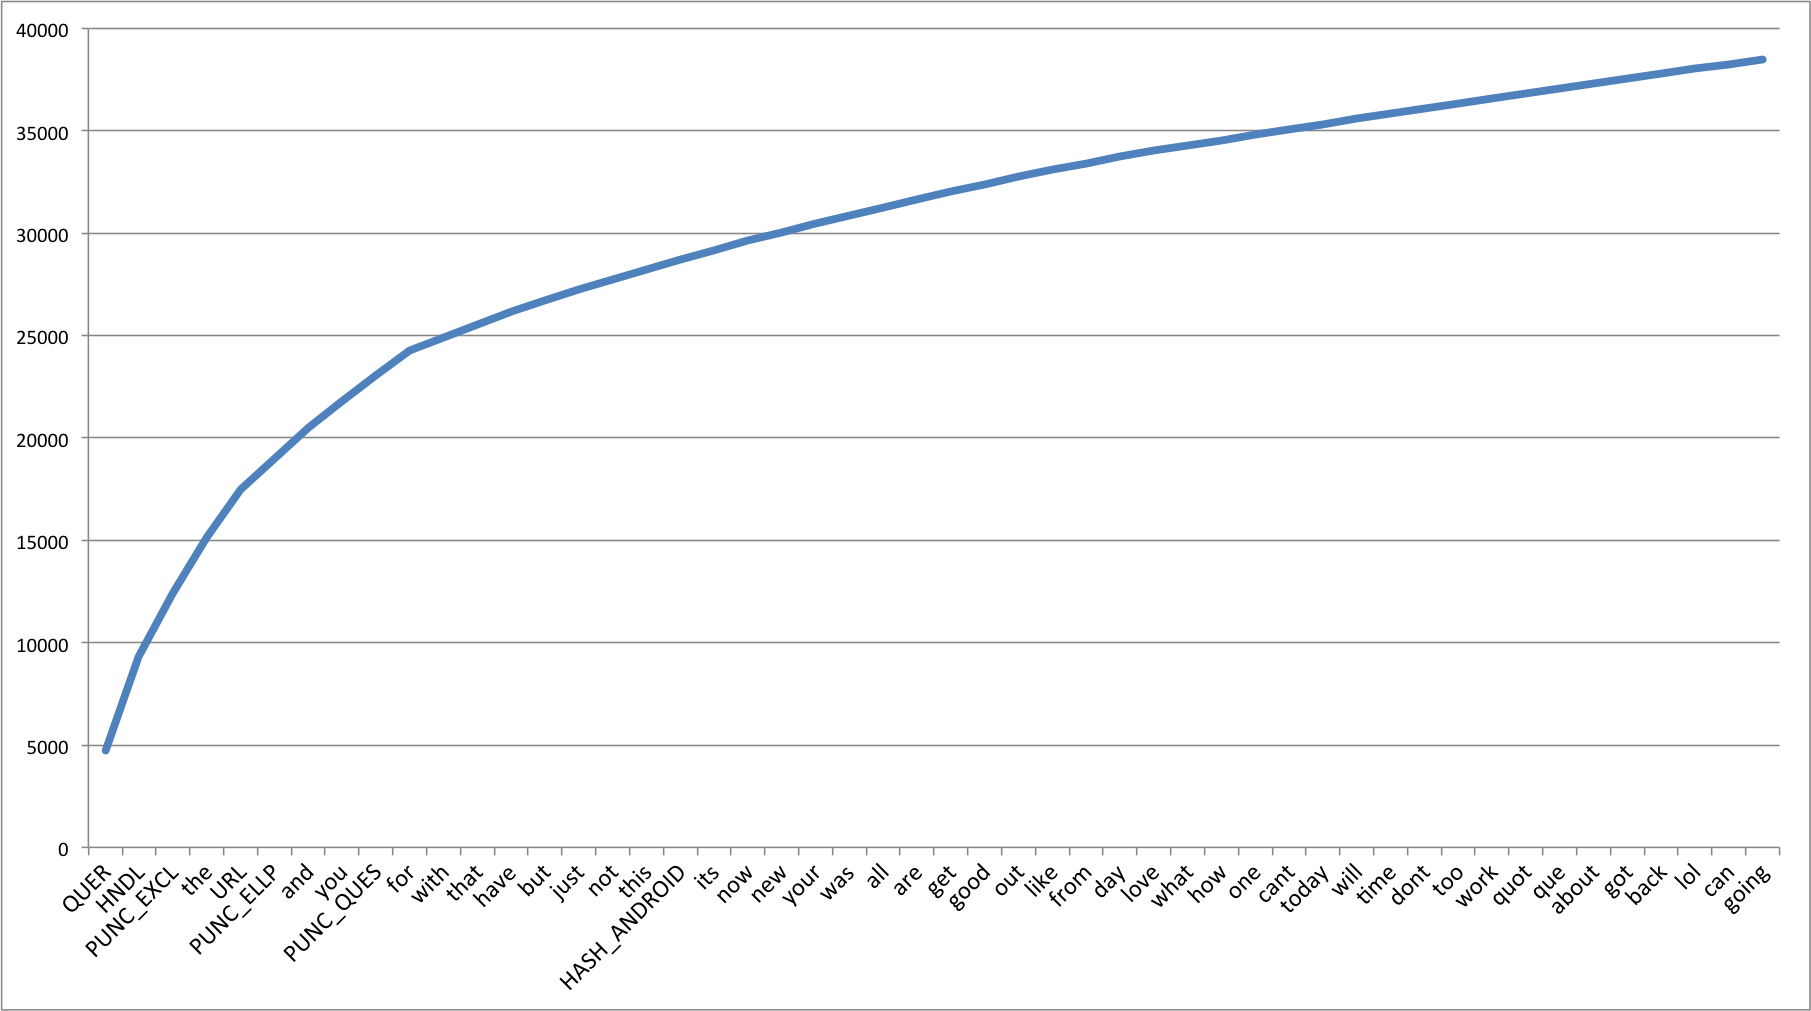
\includegraphics[width=\textwidth]{img/1grams.png}
\caption{Cumulative Frequency Plot for 50 Most Frequent Unigrams}
\label{fig:1grams}
\end{figure}

We also observe that the unigrams nicely follow Zipf’s law. It states that in a corpus of natural language, the frequency of any word is inversely proportional to its rank in the frequency table. \figref{fig:zipf} is a plot of log frequency versus log rank of our dataset. A linear trendline fits well with the data.

\begin{equation}
log( f ) = -0.9799 log( r ) + 3.9838
\end{equation}
\begin{equation}
f = 10^{3.9838} r^{-0.9799}
\end{equation}
\begin{equation}
f \propto \frac{1}{r}
\end{equation}

\begin{figure}[h!]
\centering
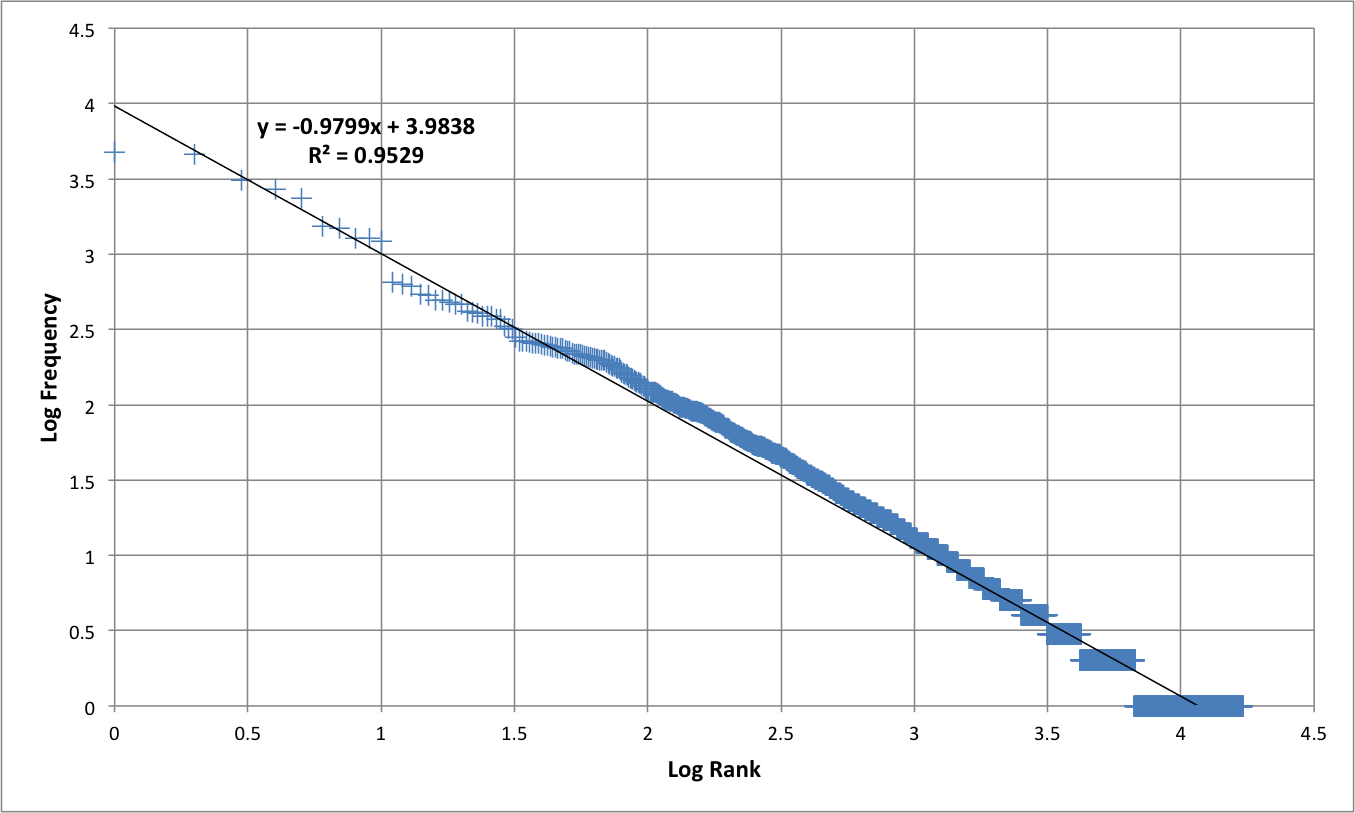
\includegraphics[width=\textwidth]{img/zipfs_law.png}
\caption{Zipf's Law - Log Frequency versus Log Rank plot for unigrams}
\label{fig:zipf}
\end{figure}


\subsubsection{N-grams}
N-gram refers to an n-long sequence of words. Probabilistic Language Models based on Unigrams, Bigrams and Trigrams can be successfully used to predict the next word given a current context of words. In the domain of sentiment analysis, the performance of N-grams is unclear. According to Pang et al., some researchers report that unigrams alone are better than bigrams for classification movie reviews, while some others report that bigrams and trigrams yield better product-review polarity classification \cite{survey}.

As the order of the n-grams increases, they tend to be more and more sparse. Based on our experiments, we find that number of bigrams and trigrams increase much more rapidly than the number of unigrams with the number of Tweets. \figref{fig:ngrams_dist_1} shows the number of n-grams versus number of Tweets. We can observe that bigrams and trigrams increase almost linearly where as unigrams are increasing logarithmically.

\begin{figure}[h!]
\centering
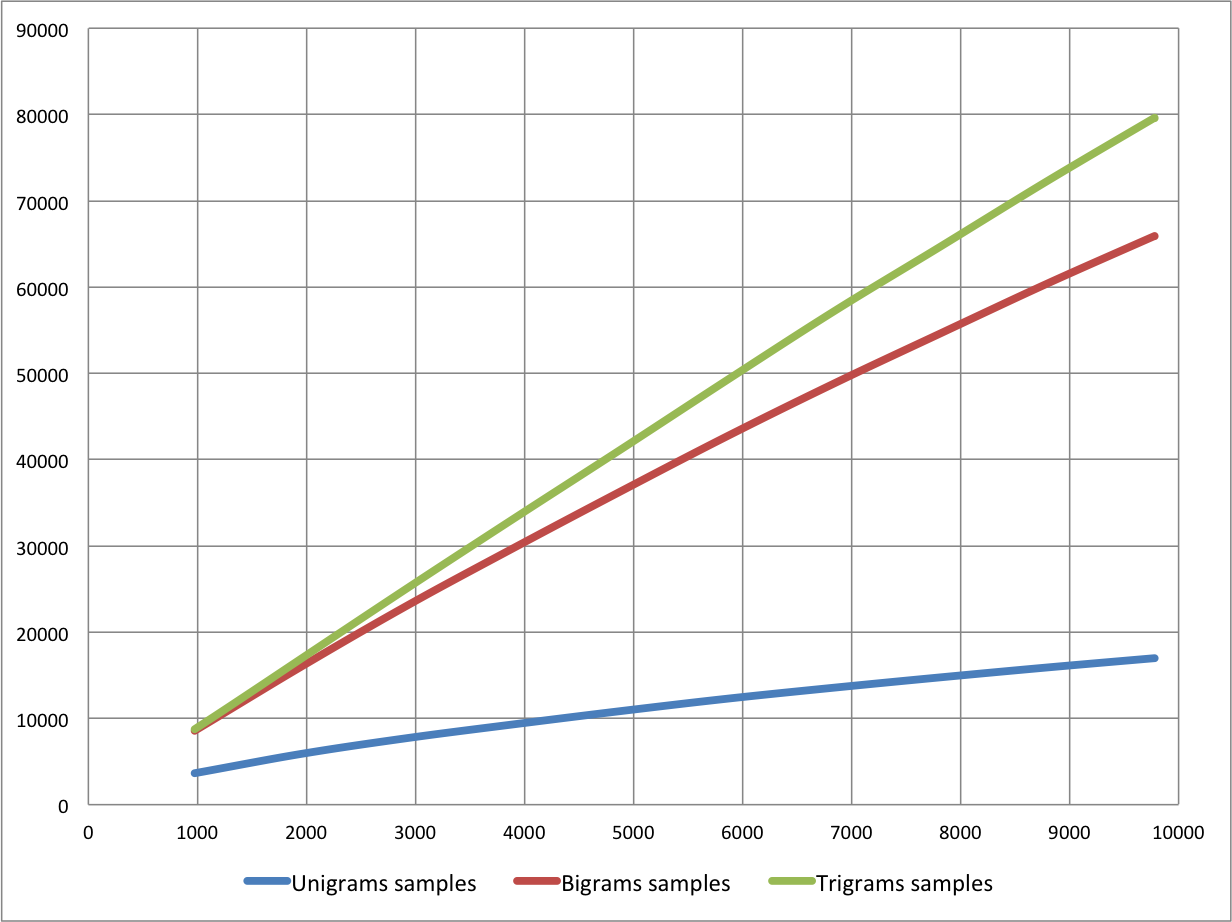
\includegraphics[width=\textwidth]{img/Ngrams_dist_1.png}
\caption{Number of n-grams vs. Number of Tweets}
\label{fig:ngrams_dist_1}
\end{figure}
%TODO: label 'ngrams growth'

Because higher order n-grams are sparsely populated, we decide to trim off the n-grams that are not seen more than once in the training corpus, because chances are that these n-grams are not good indicators of sentiments. After the filtering out non-repeating n-grams, we see that the number of n-grams is considerably decreased and equals the order of unigrams, as shown in \figref{fig:ngrams_dist_2}.

\begin{figure}[h!]
\centering
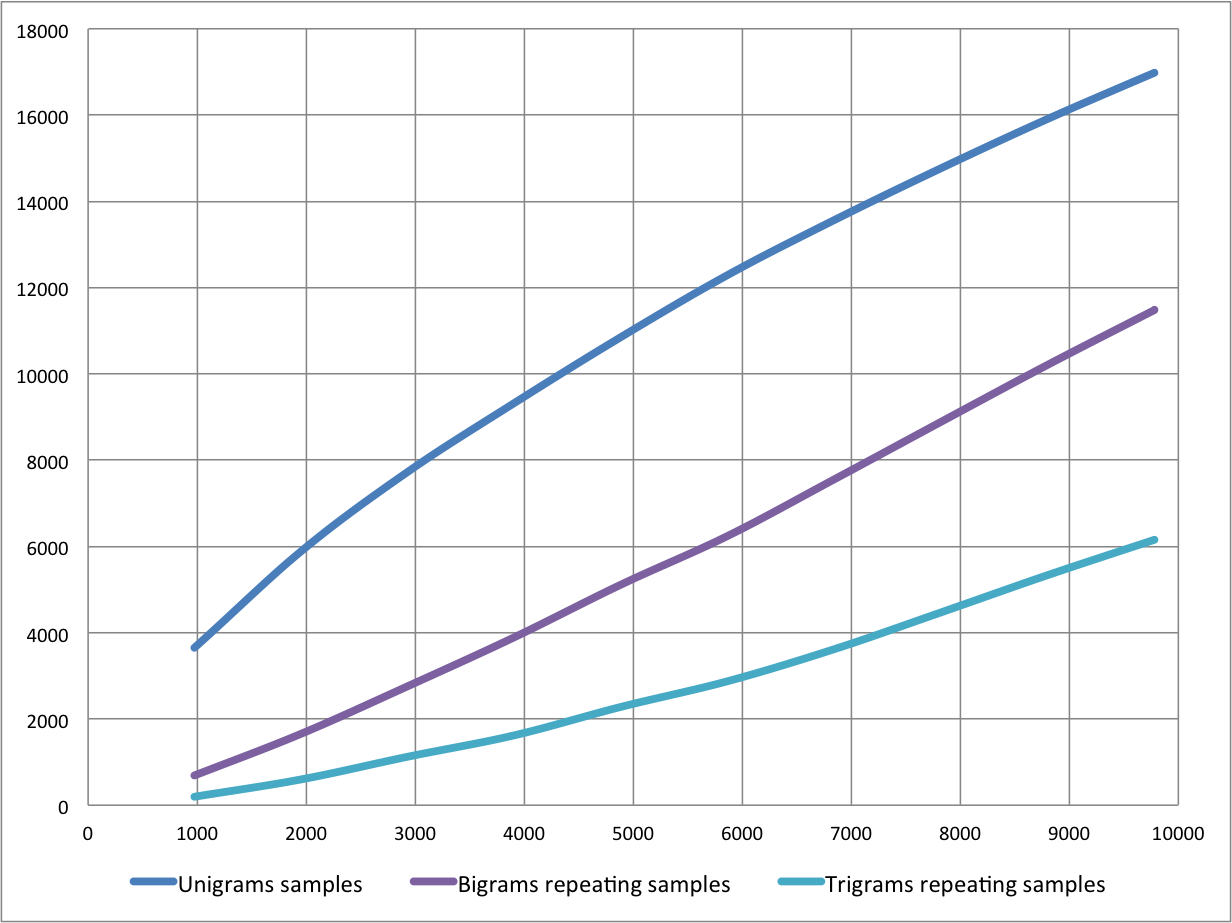
\includegraphics[width=\textwidth]{img/Ngrams_dist_2.png}
\caption{Number of repeating n-grams vs. Number of Tweets}
\label{fig:ngrams_dist_2}
\end{figure}
%TODO: label 'ngrams filtered growth'

\figref{fig:2grams} and \figref{fig:3grams} show the cumulative distribution of the most frequent bigrams and trigrams respectively.

\begin{figure}[h!]
\centering
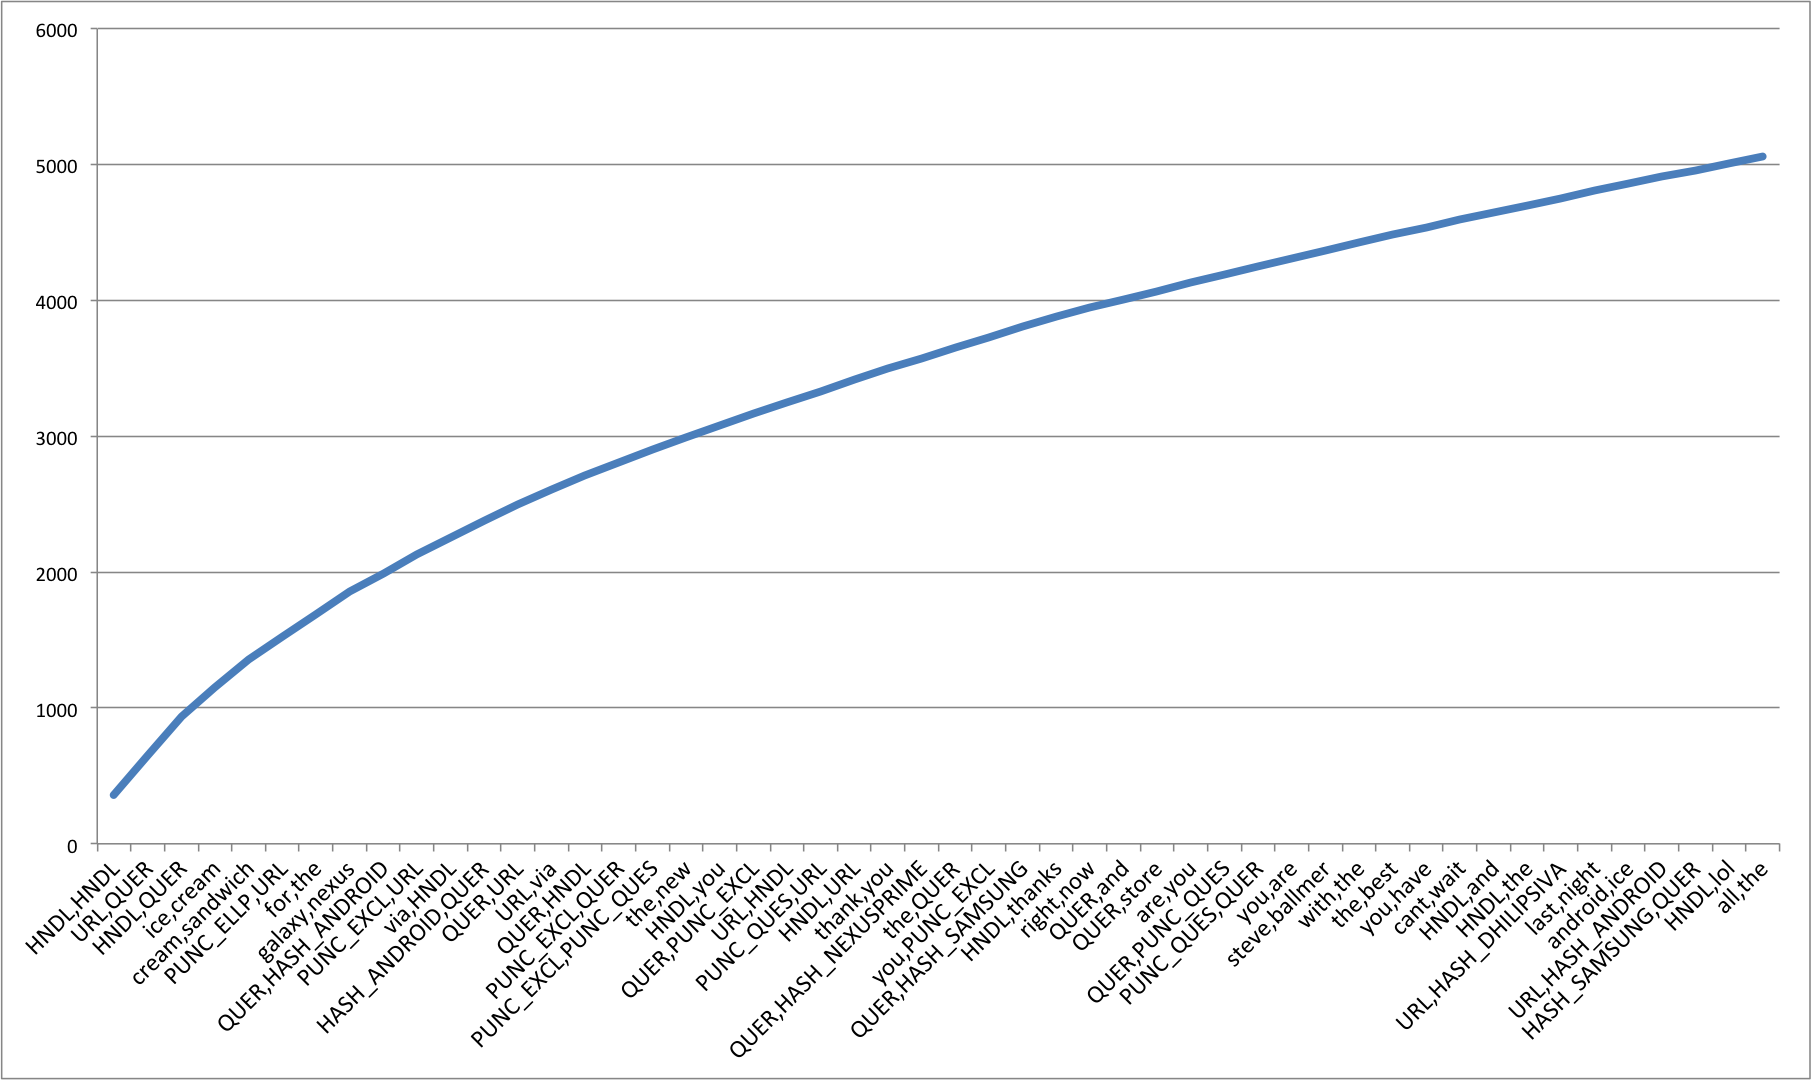
\includegraphics[width=\textwidth]{img/2grams.png}
\caption{Cumulative Frequency Plot for 50 Most Frequent Bigrams}
\label{fig:2grams}
\end{figure}

\begin{figure}[h!]
\centering
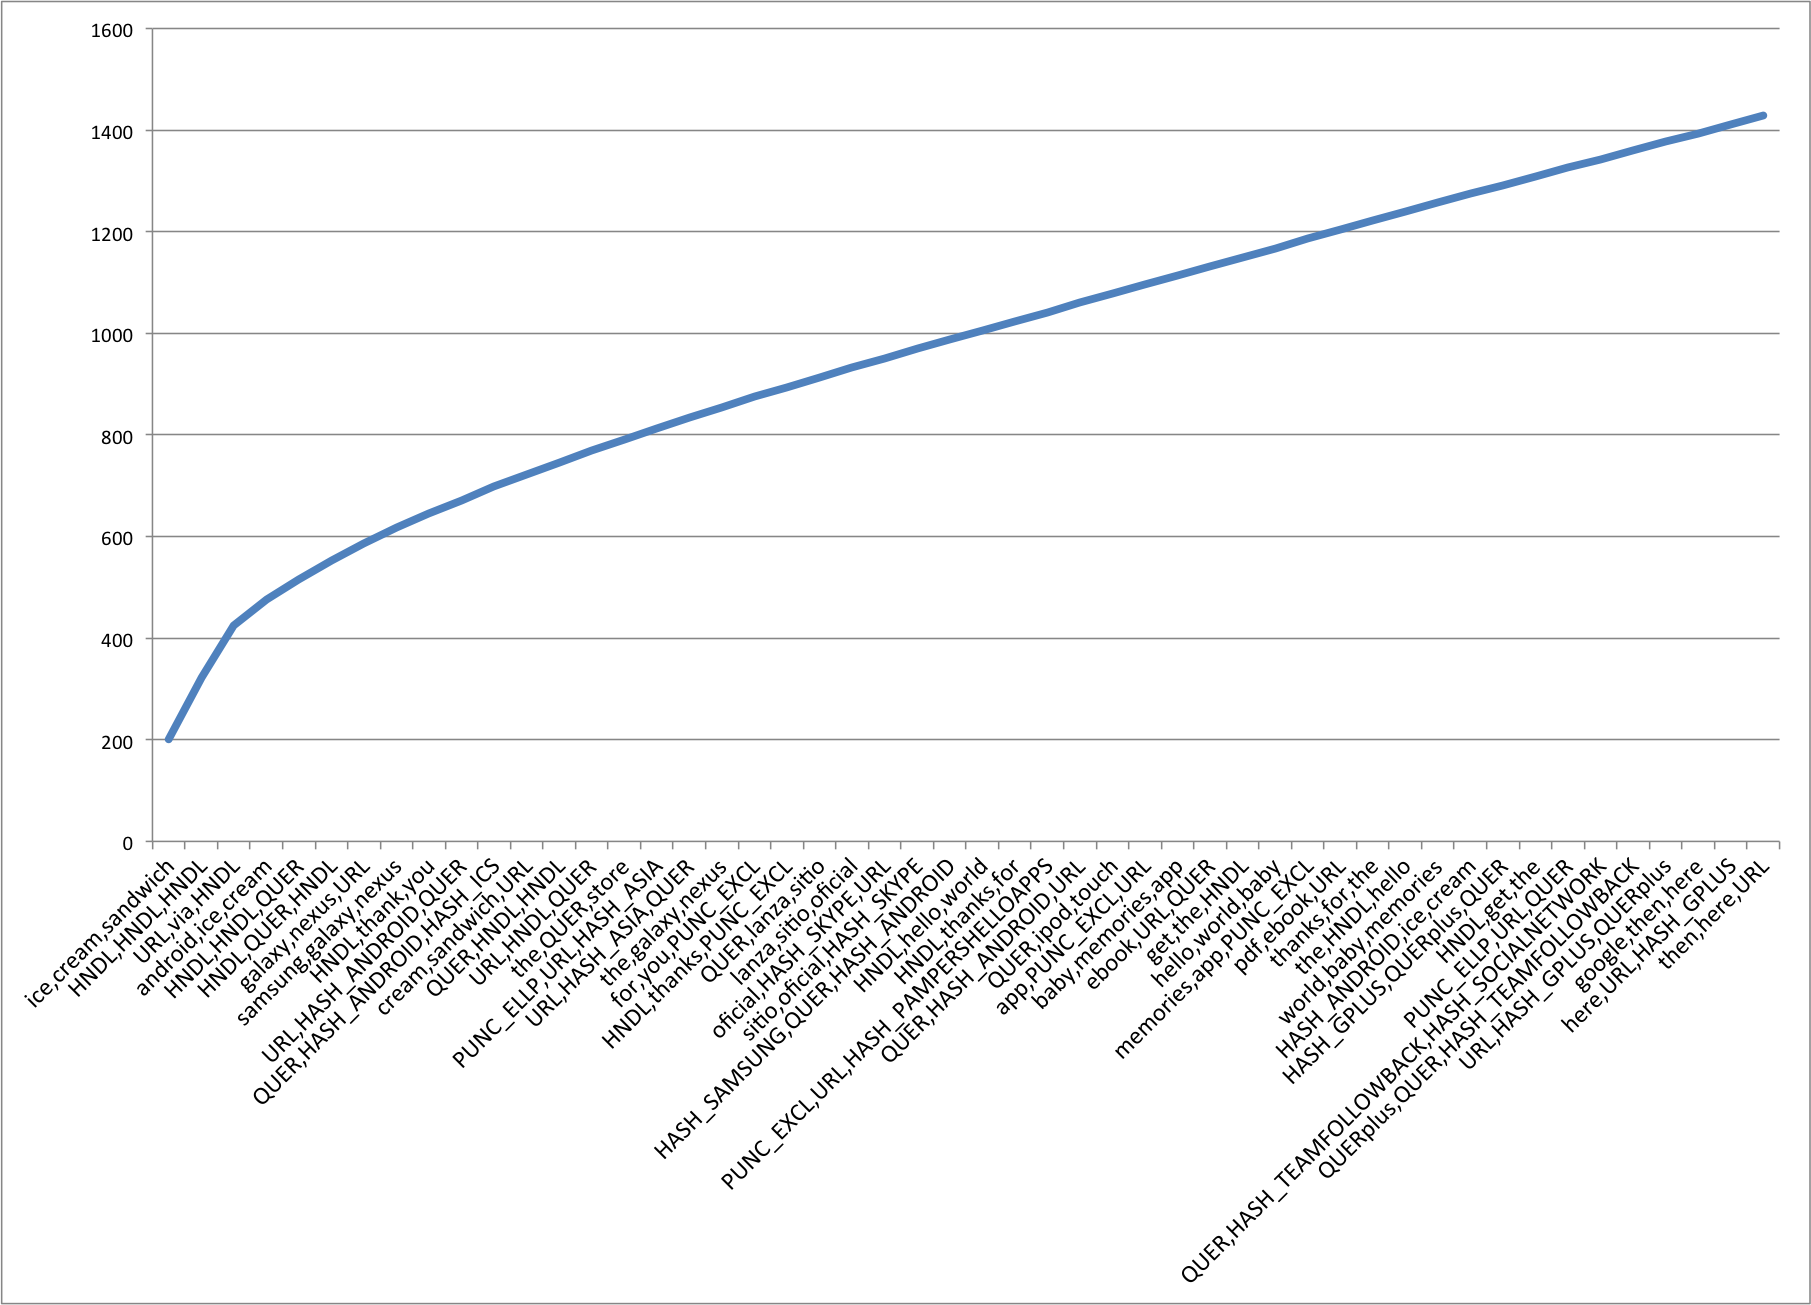
\includegraphics[width=\textwidth]{img/3grams.png}
\caption{Cumulative Frequency Plot for 50 Most Frequent Trigrams}
\label{fig:3grams}
\end{figure}

\subsubsection{Negation Handling} The need negation detection in sentiment
analysis can be illustrated by the difference in the meaning of the phrases,
``This is good'' vs. ``This is not good'' However, the negations occurring in
natural language are seldom so simple. Handling the negation consists of two
tasks – Detection of explicit negation cues and the scope of negation of these
words.

Councill et al. look at whether negation detection is useful for sentiment
analysis and also to what extent is it possible to determine the exact scope of
a negation in the text \cite{CMV}. They describe a method for negation detection
based on Left and Right Distances of a token to the nearest explicit negation
cue.

\subsubsection*{Detection of Explicit Negation Cues} To detect explicit negation
cues, we are looking for the following words in \tabref{tab:negation}. The
search is done using regular expressions.

\begin{table}[h!]
\centering
\begin{tabular}{|l|l|l|}
\hline
S.No. & Negation Cues \\\hline
1.  & never \\
2.  & no \\
3.  & nothing \\
4.  & nowhere \\
5.  & noone \\
6.  & none \\
7.  & not \\
8.  & havent \\
9.  & hasnt \\
10.  & hadnt \\
11.  & cant \\
12.  & couldnt \\
13.  & shouldnt \\
14.  & wont \\
15.  & wouldnt \\
16.  & dont \\
17.  & doesnt \\
18.  & didnt \\
19.  & isnt \\
20.  & arent \\
21.  & aint \\
22.  & Anything ending with ``n't'' \\\hline
\end{tabular}
\caption{Explicit Negation Cues}
\label{tab:negation}
\end{table}

\subsubsection*{Scope of Negation} Words immediately preceding and following the
negation cues are the most negative and the words that come farther away do not
lie in the scope of negation of such cues. We define left and right negativity
of a word as the chances that meaning of that word is actually the opposite.
Left negativity depends on the closest negation cue on the left and similarly
for Right negativity. \figref{fig:negation} illustrates the left and right
negativity of words in a tweet.

\begin{figure}[h!]
\centering
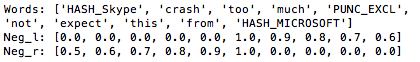
\includegraphics[width=\textwidth]{img/negation.png}
\caption{Scope of Negation}
\label{fig:negation}
\end{figure}


